\section{Annulus homeomorphisms and billiard map}

Let $\mathbb{ A}=\mathbb{T}^1\times [0,\pi]$ be the annulus (or cylinder).

Let $\gamma:\mathbb{T}^1\to\mathbb{R}^2$ a smooth convex curve, i.e., $\Gamma=\gamma(\mathbb{T}^1)$ bounds a convex region. 

 

Let $p\in \Gamma$ and consider a line $\ell_p$ passing through $p$ and making an angle $\theta\in (0,\pi)$ with the tangent line $T_p\Gamma$. The second point of intersection of $\ell_p$ with $\Gamma$ will be denoted by $p'$, and the angle of the line $\ell_p$  with $T_{p'}\Gamma$ will be denoted by $\theta'$.

Repeat this construction starting in $p'$ and   line $\ell_{p'}$ making angle $\pi-\theta'$ with the tangent line $T_{p'}\Gamma$. As before we will obtain $p''$ and $\theta''$. 

The billiard map is defined as
$T:\mathbb{A} \to\mathbb{A}]$,  $T(p,\theta)= (p',\theta')$, with $T(p,0)=(p,0)$ and $T(p,\pi)=(p,\pi)$, where $p=\gamma(s)$ and $p'=\gamma(s')$. See \cref{fig:appC-billiard-map}.
\begin{figure}
    \centering
    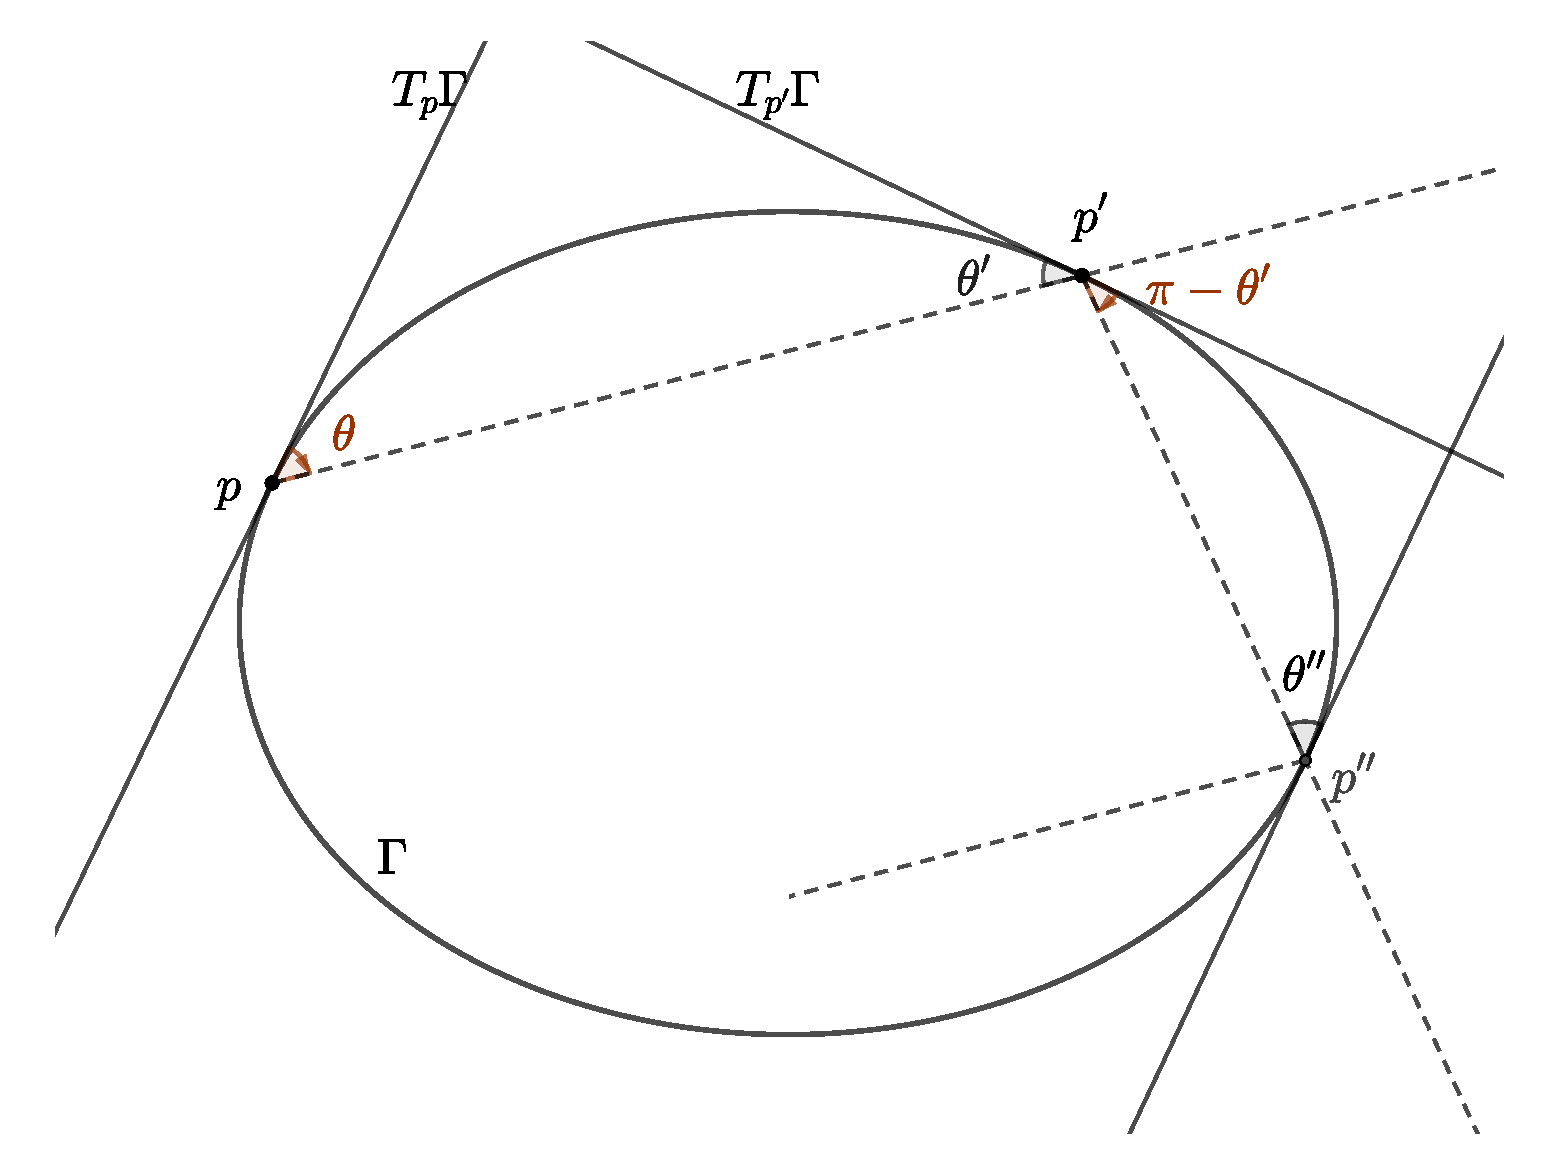
\includegraphics[scale=0.4]{zappC/pics/pics_appC_160bilharmapanel.pdf}
    \caption{Billiard map of a convex billiard}
    \label{fig:appC-billiard-map}
\end{figure}

The following result is due to Birkhoff \cite{birkhoff1922}.

\begin{theorem} Consider the area form $\Omega=\sin\theta ds\wedge d\theta$. Then $T^{*}\Omega=\Omega$, i.e., the map $T$ preserves area.
\end{theorem}

\begin{proof} See \cite{sergei2002}.\end{proof}

